\chapter{Antenna Arrays}
In the previous section, we derived a relationship between the current distribution and radiation pattern and with that relationship we can get the desired radiation pattern by manipulating the current distribution. However, we cannot modify this distribution without affecting the terminal characteristics, therefore in this section, we would study the antenna arrays as a flexible way of controlling the current distribution without affecting the terminal characteristics.

Antenna arrays is a large number of antennas with predefined terminal characteristics that are placed in the vicinity of each other and are excited simultaneously. Thus, we get a field which is the superposition of the individual fields and it results to a modified radiation pattern. Essentially, this arrangement will decouple the terminal characteristics and the radiation pattern but it is important to note that when two antennas are brought in the vicinity of each other the terminal characteristics will be affected slightly if the distance between them is more than $ \frac{\lambda}{2}$. So if the antenna elements are separated with a distance of $ \frac{\lambda}{2} $ the terminal characteristics practically remain unchanged. Hence, the antenna array provides flexibility in designing the desired radiation pattern. Let's consider a situation where we want to transmit(or receive whichever case) at a frequency. First, we find a suitable antenna with proper impedance and bandwidth characteristics, maybe a dipole for instance, and match data to it over the bandwidth.

This is now the basic element, so to create an array we reproduce this base element at different locations in space so that each antenna element is the best radiating element at that frequency, for that bandwidth and superposition of all the radiation from these antenna elements of similar types gives the desired radiation pattern.

It is to great advantage that the antenna arrays consist of identical antenna elements, this simplifies the analysis and eventually, the radiation pattern gets modified which is decided by the array characteristics.

Now lets consider a collection of dipole antennas arranged in space as shown in Figure~\ref{52.1} with current, $I_1$ to $I_5$ which flows through them.
\begin{figure}[h]
\centering
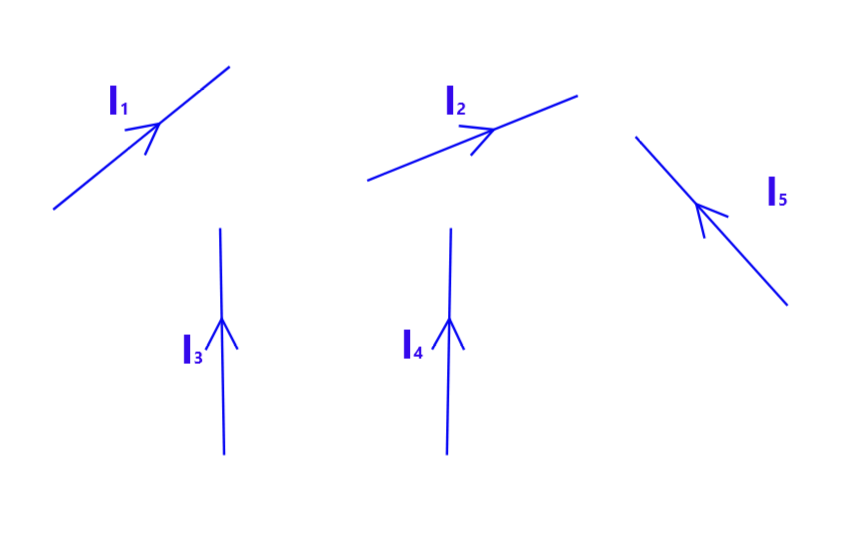
\includegraphics[height=5cm]{/graphics/fig52_1}
\caption{}
\label{52.1}
\end{figure}

This arrangement is an array, however our analysis involves the superposition of the electric field of each antenna element at a distance that is very far away. So again this arrangement is not of any advantage as far as radiation pattern is concerned. Therefore, these elements are oriented in the same direction so that they have identical radiation characteristics as a function of $\theta$ and $\phi$.

Now, lets identify the quantities which control the radiation pattern for any given array arrangement. They are as follows;
\begin{enumerate}[(i)]
\item \textbf{Spatial configuration of the antenna elements}: This is the distribution of elements in space. For instance, for a line we have a linear configuration. 
\item \textbf{Location of the antenna elements}: This is the spacing between the different elements and it varies for different configurations such as the linear or circular configuration.
\item \textbf{Relative Amplitude of the antenna elements}.
\item\textbf{Phase of antenna elements}.
\item \textbf{Radiation pattern of basic element}: For instance, if we have a basic element as a dipole, it has a null along its axis and so a linear array of these elements oriented in the same direction will also have a null along the axis.
\end{enumerate}
Generally, a configuration will contain a given number of antenna elements given by $N$. If for instance we decide on the configuration and the radiation pattern of the antenna elements,  then there are three quantities left to control. Therefore, for $N$ elements, each quantity can be varied in ($N-1$) ways since we are considering the relative measure and it is essentially the degree of freedom. So essentially for the three quantities we have $3(N-1)$ degree of freedom which is a very large number. In practice we do not require this large number of degree of freedom so we decide on some more quantities such as choosing uniform arrays, also choosing the same amplitude and then the radiation characteristics is controlled by only the phase variation of the antenna elements.

\section{Two element array}
Lets first examine the simplest possible array with just 3 degrees of freedom i.e the spacing between the elements, the relative amplitude and the phase variation and we will observe the effect these quantities have on the radiation pattern. Figure~\ref{52.2} shows two elements linearly arranged along the horizontal axis called the array axis or axis of the array. For a broad radiation (close to an isotropic radiation) we will consider a Hertz dipole whose radiation pattern is symmetric in the H-plane ($\phi$ direction) as shown. These two Hertz dipole are perpendicular to the plane of the paper and have current $I_1$ and $I_2$ with phases $\delta_1$ and $\delta_2$ respectively, flowing through them. We would like to examine the radiation pattern at a far away distance called the observation point, measured from the axis of the array given by $\phi$, while varying three quantities
\begin{figure}[h]
\centering
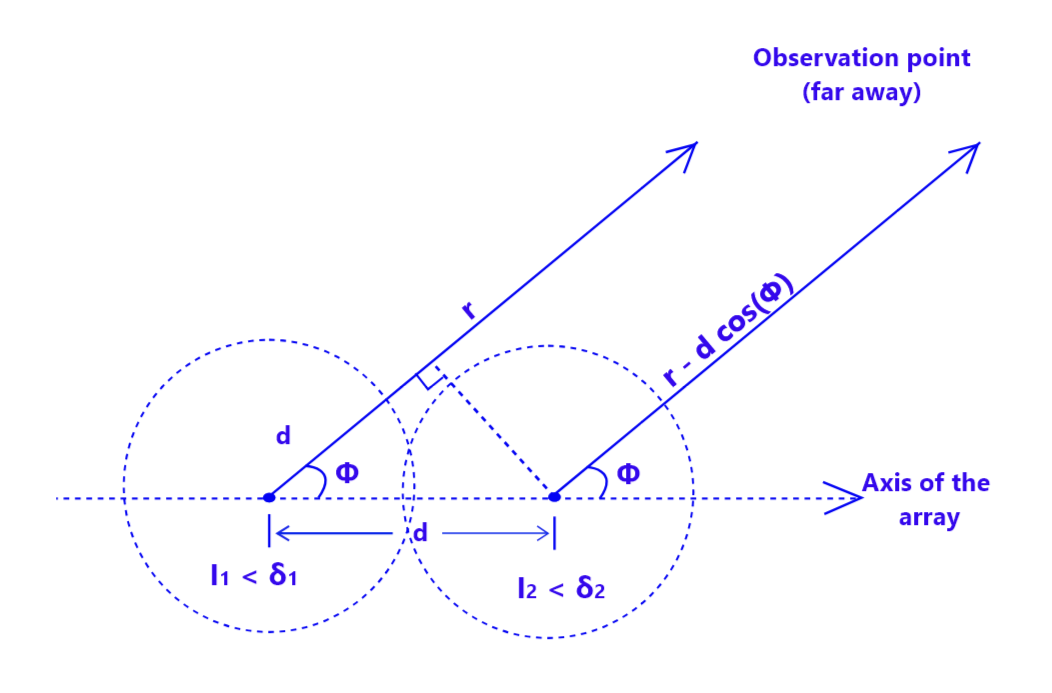
\includegraphics[height=5cm]{/graphics/fig52_2}
\caption{}
\label{52.2}
\end{figure}

which are the separation between the antenna elements given by d, the relative amplitude $\frac{I_2}{I_1}$ and the phase difference ($\delta_2$-$\delta_1$). The distance from element 1 is given as r and the distance from element 2 is $r-d\cos\phi$ and the fields due to each of the elements is given as 
$$
\text{Electric field for element 1} \quad E_1 = k I_{1} e^{j\delta_1}  \dfrac{e^{-j\beta r}}{r}  
$$ 
$$
\text{and Electric field for element 2} \quad E_2 =k I_{2} e^{j\delta_2} \dfrac{e^{-j\beta(r-dcos\phi)}}{r-dcos\phi}% recheck equation
$$
$$
\text{$E_2$ can be approximated to} \quad E_2 = k I_{2}
e^{j\delta_2} \dfrac{e^{-j\beta(r-dcos\phi)}}{r}  %recheck
$$
So the total field which is the superposition of the individual fields of the elements at the observation point is given as ;
$$
\quad E = E_1 + E_2
$$           
\begin{equation}
\label{32}                   
=  \quad k I_{1} e^{j\delta_1}\dfrac{e^{-j\beta r}}{r} + k I_{2} e^{j\delta_2} \dfrac{e^{-j\beta(r-dcos\phi)}}{r} %recheck                     
\end{equation}
Since we are concerned with the radiation pattern of the arrangement which is the relative variation of the electric field as a function of angle $\phi$ we define a constant   
$$
\quad k_o =\dfrac{ke^{-j\beta r}}{r}  %recheck 
$$
So, the total electric field in Equation~\ref{32} becomes 
$$
\quad E = k_o I_1e^{j\delta_1} + k_o I_2e^{j\delta_2} e^{j\beta dcos\phi}
$$
$$
\quad = k_o \{I_1 e^{j\delta_1} + I_2 e^{j\delta_2} e^{j\beta dcos\phi}\}
$$
\text {We rewrite the expression in terms of }\quad $\dfrac{I_2}{I_1}$  {and}  ($\delta_2 - \delta_1$) . So, 
\begin{equation}
\label{33}
\quad E = k_o I_1 e^{j\delta_1} \{1 + \dfrac{I_2}{I_1} e^{j (\delta_2 - \delta_1)} e^{j\beta dcos\phi}\}
\end{equation} 
The expression shows that the electric field (or the normalized electric field or radiation pattern) can be controlled by either varying $\dfrac{I_2}{I_1}$ , d and the phase difference ($\delta_2 - \delta_1$) which essentially are the degrees of freedom.
\subsection{Effect of variation of $d$}
Lets examine the effect of the variation of the separation between these elements d. Without losing generality, we would choose the quantities $\dfrac{I_2}{I_1} = 1, \delta_2 - \delta_1 = 0 , I_1 =1 $ and $\delta_1 = 0 $ and as such Equation~\ref{33} reduces to
$$
\quad E = k_o \{1 + e^{j\beta dcos\phi}\}  \text{ which is rewritten as ;} 
$$
$$
= k_o e^{j\frac{\beta d}{2} cos\phi} \{e^{-j\frac{\beta d}{2} cos\phi} + e^{j\frac{\beta d}{2} cos\phi}\} 
$$ 
we recall $ e^{jx} + e^{-jx} = 2cosx $ so;
\begin{equation}
\quad E = k_o  e^{j\dfrac{\beta d}{2} cos\phi} \times 2 cos \{\dfrac{\beta d}{2} cos\phi\}   
\end{equation} 
The radiation pattern is $ cos\{\dfrac{\beta d}{2} cos\phi\} $ because 2$k_o $ is a constant and the term $e^{\frac{\beta d\cos\phi}{2}}$ is a phase term. 

So Radiation pattern
$$F(\phi) = \cos\left(\frac{\beta d\cos\phi}{2}\right)$$
For the radiation pattern $ F(\phi) = 1 $ when $\phi = $ odd multiples of $ \dfrac{\pi}{2} $ i.e $ \pm \dfrac{\pi}{2} $ , $ \pm \dfrac{3\pi}{2} $ , $ \pm \dfrac{5\pi}{2} $ ,... which is along the vertical axis. Since $ \phi $ varies from 0 to $ \pi $ then the radiation pattern is maximum when $ \phi = \dfrac{\pi}{2} $ . Therefore if we consider two element array the maximum occurs when $ \phi = \dfrac{\pi}{2} $ . Also, we have nulls i.e $ F(\phi) = 0 $ when $ \dfrac{\beta d}{2} cos\phi = $ odd multiples of $ \dfrac{\pi}{2} $  i.e  $ \pm \dfrac{\pi}{2} $ , $ \pm \dfrac{3\pi}{2} $ , $ \pm \dfrac{5\pi}{2} $ ,... substituting $ \beta = \dfrac{2\pi}{\lambda} $ then $ \dfrac{\beta d}{2} cos\phi = \pm \dfrac{\pi}{2} $ , $ \pm \dfrac{3\pi}{2} $ , $ \pm \dfrac{5\pi}{2} $ , $ \pm \dfrac{7\pi}{2} $ ,... $ $ is rewritten as $ \dfrac{2\pi}{\lambda} \dfrac{d}{2} cos \phi = \pm \dfrac{\pi}{2} $ , $ \pm \dfrac{3\pi}{2} $ ... therefore,
\\ $ cos \phi = \pm \dfrac{\lambda}{2d} , \pm \dfrac{3\lambda}{2d} , \pm \dfrac{5\lambda}{2d} $ ,... which gives the angle $ \phi $ for the direction of the nulls given the value of d. Now for the range of values of $ \phi $ when $ cos\phi $ equals to values from -1 to +1\footnote{as $ \phi $ varies from (0 - $ \pi $ )} , will give the physical nulls. It should be noted that if we increased d for a given value of $ \lambda $ then we would have more directions of nulls. For instance if $ d < \dfrac{\lambda}{2} $ , then we would get a radiation pattern with no nulls but if $ d = \lambda $ , only the first term $ \pm \dfrac{\lambda}{2d} $ gives $ \pm \dfrac{1}{2} $ which gives two nulls that lies within -1 to +1, which is equivalent to two nulls  at $ \phi = cos^{-1} \{\pm \dfrac{1}{2} \}  $  

Also at $ d = 2 \lambda $ , the first term gives $ \pm \dfrac{1}{4} $ which is permissible and the second term also gives  $ \pm \dfrac{3}{4} $ which is also permissible  and therefore we have four nulls at the angles $ \phi = cos^{-1} \{\pm \dfrac{1}{4} \}  $ and $ cos^{-1} \{\pm \dfrac{3}{4} \}  $ 
The other terms give values greater than -1 to +1 .

Therefore, for a given current excitation (for a given amplitude ratio for the currents through the elements) and as well as for a given phase difference between the currents of the antenna element, as the separation between the elements increases the number of nulls go on increasing, which means the larger the spacing of the antenna elements the number of nulls in the radiation pattern increases.
\begin{figure}[h]
\centering
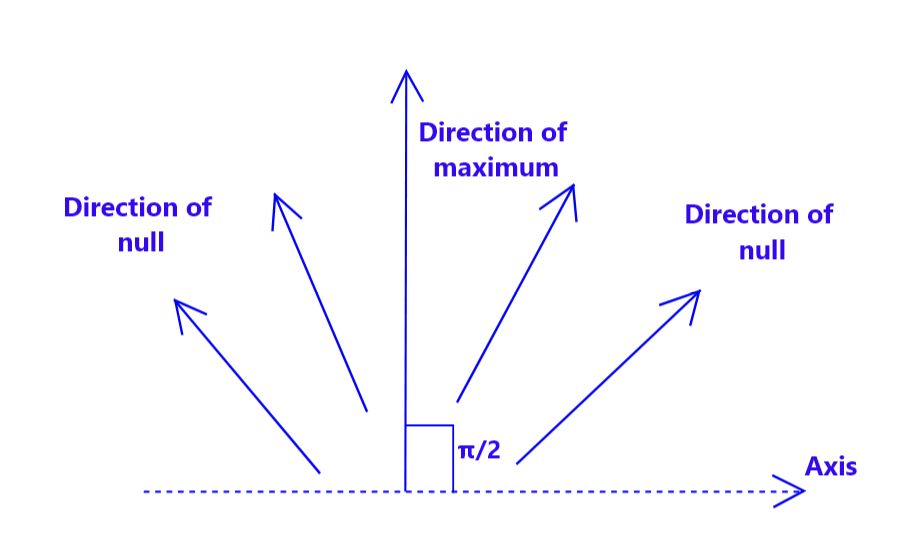
\includegraphics[height=5cm]{/graphics/fig52_3}
\caption{}
\label{52.3}
\end{figure}

We recall that in between two consecutive nulls there exist a maximum. Then from Figure~\ref{52.3} we can say the direction of maximum should have the main beam and other beams that exist within the nulls should be locally maxima (side lobes). However, this is not the case here, what we have is that the radiation is maximum in all direction but has a radiation pattern with multiple nulls therefore the pattern is sectorized. We conclude that as the spacing increases, the number of nulls increase and the number of sectors increase as well . Hence, if we want no nulls in the radiation pattern then $ d < \dfrac{\lambda}{2} $ , however this choice is not very desirable and there are constraints from the radiation pattern which we will see later.

\subsection{Effect of variation in $ \left( \dfrac{I_2}{I_1} \right) $ } 
Now lets examine the effect of the variation of the ratio of the currents in the antenna elements. Without losing generality, we make $ d = \lambda ,  \delta_2 - \delta_1 = 0 , I_1 =1 $ and $\delta_1 = 0 $ . Then $ \beta dcos\phi $ for $ ( \beta = \dfrac{2 \pi}{\lambda} \text{ and }  d = \lambda) $ equals $ \dfrac{2 \pi}{ \lambda } \lambda cos \phi = 2 \pi cos \phi $ . From Equation~\ref{33}
$$
\quad  E = k_o I_1 e^{j \delta_1} \{1 + \left( \dfrac{I_2}{I_1}\right) e^{j( \delta_2 - \delta_1)} e^{j \beta dcos\phi}\} 
$$
becomes
\begin{equation}
\quad E = k_o \{ 1 +  \left(\dfrac{I_2}{I_1}\right) e^{j 2 \pi cos\phi}  \}
\end{equation}
From the equation we observe that as $ \phi $ varies  the phase of the electric field varies. So lets consider the cases where $ e^{j 2 \pi cos\phi} = \pm 1 $ . Hence when $ 2 \pi cos\phi = 0, 2 \pi, 4 \pi, 6 \pi, ... $ then  $ e^{j 2 \pi cos\phi} = 1\ (\text{since}\ e^{j \theta} = cos\theta + j sin\theta) $ . However, range of $ \phi $ is from 0 to $ \pi $ so $ e^{j 2 \pi cos\phi} $ will be 1 when $ cos\phi = 0 $ i.e $ \phi = \dfrac{ \pi }{ 2 } $ and we have $ E  = k_o \left\{ 1 + \dfrac{I_2}{I_1} \right\} $ .
Also lets examine when  $ e^{j 2 \pi cos\phi} = - 1 $ which is when $ 2 \pi cos\phi = \pi, 3 \pi, 5 \pi,... $ . Also, since the range of $ \phi $ is limited then $ e^{j 2 \pi cos\phi} = - 1 $ when $ cos\phi = \dfrac{ 1 }{ 2 } $ (as the other values are greater than 1 i.e $ \dfrac{ 3 }{ 2 }, \dfrac{ 5 }{ 2 }, ... $ ) which is when $ \phi = \dfrac{ \pi }{ 3 } $ and we have $ E  = k_o \left\{ 1 - \dfrac{I_2}{I_1} \right\} $ . So $ E  = k_o \left\{ 1 + \dfrac{I_2}{I_1} \right\} $ is the maximum value for electric field as  $ \phi $ varies and $ E  = k_o \left\{ 1 - \dfrac{I_2}{I_1} \right\} $ is the minimum value which is seen in the radiation pattern. However, the important observation to note is that if the ratio $\frac{I_2}{I_1}$ is not one ie. the two currents are not equal there is no complete cancellation of the fields which means there is no complete constructive or destructive interference. Essentially when $ I_2 \neq I_1 $ there will never be a null in the radiation pattern instead the complete amplitude of the radiation is only reduced to a certain value that is not zero. In conclusion, we say that the depth of the nulls is controlled by the current amplitude of the two elements $ \dfrac{ I_2 }{ I_1 } $.

\subsection{Effect of phase difference $ ( \delta_2 - \delta_1 ) $ }
Again, without losing generality let $ \dfrac{ I_2 }{ I_1 } = 1, I_1 = 1, \delta_1 = 0 \text{ and } \delta_2 = \delta $ . So, from Equation~\ref{33};
$$
\quad E = k_o \{ 1 + e^{j ( \beta dcos\phi + \delta)} \}
$$
$$
\quad = k_o e^{j \dfrac{ \beta dcos\phi + \delta }{ 2 } } \left\{ e^{ -j \dfrac{ \beta dcos\phi + \delta }{ 2 } } + e^{j \dfrac{ \beta dcos\phi + \delta }{ 2 } } \right\}
$$
\begin{equation}
\quad = k_o e^{j \dfrac{ \beta dcos\phi + \delta }{ 2 } } \times 2 cos \left( \dfrac{ \beta dcos\phi + \delta }{ 2 } \right) 
\end{equation}
which again gives the normalized electric field ( radiation pattern ) as $ cos \left( \dfrac{ \beta dcos\phi + \delta }{ 2 } \right) $ where $  e^{j \dfrac{ \beta dcos\phi + \delta }{ 2 } } $ is the phase term and $ 2 \text{ and } k_o $ are constants. The maximum radiation we get corresponds to $  cos \left( \dfrac{ \beta dcos\phi_ {\textnormal{max}} + \delta }{ 2 } \right) = \pm 1 ;   \left( \dfrac{ \beta dcos\phi_ {\textnormal{max}} + \delta }{ 2 } \right) = 0, \pi, 2 \pi,... $ \\ Therefore, $\beta dcos\phi_ {\textnormal{max}} + \delta = 0 $ \footnote{considering only the first term on the range (0, $\pi$, $2\pi$, ...)}\\
$ cos\phi_ {\textnormal{max}} = \dfrac{ - \delta }{ \beta d } $ , which gives the direction of maximum radiation. 

What the expression means is that if we change the value of $\delta $ given the value $d $ then the direction of maximum radiation changes. Therefore, by changing the phase difference of the two elements essentially the direction of maximum radiation changes . For instance if $ \delta = 0 $ then $ \phi_{\textnormal{max}} = \dfrac{ \pi }{ 2 } $ . Also, if $ \delta = \pm \beta d \text{ i.e } cos\phi_{\textnormal{max}} = \pm 1 $ and $ \phi_{\textnormal{max}} = \pi \text{ or } 0 $ . So as the phase difference changes the direction of the maximum beam changes from $ 0 \text{ to } \dfrac{ \pi }{ 2 } \text{ to } \pi $ ( which corresponds to $ \delta = - \beta d , 0 , \text{ and } \beta d $ \text{ respectively }) as shown in Figure~\ref{52.4}.
\begin{figure}[h]
\centering
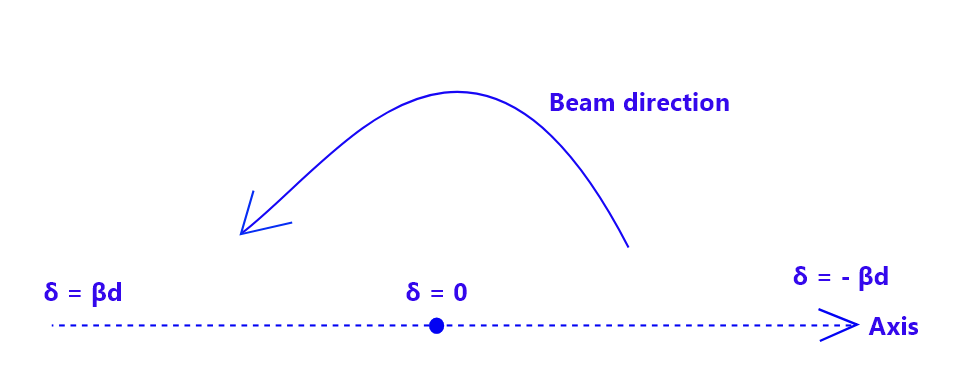
\includegraphics[width=1\linewidth]{/graphics/fig52_4}
\caption{}
\label{52.4}
\end{figure}

Hence, the phase difference between elements essentially has the effect of rotating the radiation pattern i.e changing the beam direction of the antenna array.

In conclusion each of the three parameters; ratio of the  current, amplitude, the phase difference and the inter element spacing has a unique effect on the radiation pattern and it will be useful in discussing the next topic where we would treat $ N $ elements arrays of which these parameters would be adjusted to get the desired radiation pattern.